\documentclass{article}

% Language setting
\usepackage[english]{babel}

% Page layout
\usepackage[letterpaper,top=2cm,bottom=2cm,left=3cm,right=3cm,marginparwidth=1.75cm]{geometry}

% Math, graphics, and links
\usepackage{amsmath}
\usepackage{amssymb}
\usepackage{amsthm}
\usepackage{graphicx}
\usepackage{listings}
\usepackage[colorlinks=true, allcolors=blue]{hyperref}

\lstset{
  basicstyle=\ttfamily\footnotesize,
  breaklines=true,
  breakatwhitespace=false,
  columns=fullflexible,
  keepspaces=true
}

\newtheorem{definition}{Definition}
\newtheorem{proposition}{Proposition}

\title{Neural Network in C++ Notes}

\author{Ethan Cochran}
\date{\today}

\begin{document}
\maketitle

\begin{abstract}
These notes derive and document a small fully connected neural network implemented from scratch in C++. The network is a configurable multilayer perceptron with dense affine layers, `tanh` hidden activations, a sigmoid binary output, and binary cross-entropy loss. The main training example is XOR, which requires a hidden layer because it is not linearly separable.

The goal is not to build a general machine-learning framework, but to understand each numerical step: parameter shapes, forward propagation, stable loss computation, manual backpropagation, batch gradient averaging, finite-difference gradient checking, and gradient-descent training. Every formula in these notes should correspond directly to code in the project.    
\end{abstract}

\tableofcontents

\pagebreak

\section{Overview}

% Purpose: construct a multilayer perceptron from scratch in C++.
% Support an arbitrary number of fully connected layers and layer widths.
% Implement initialization, forward propagation, loss evaluation,
% backpropagation, gradient checking, and gradient-descent training.
% Use XOR as a small nonlinear classification test.
% No machine-learning or automatic-differentiation libraries are used. 

The goal of this lab is to translate the mathematical theory of neural networks into a complete implementation in C++. A fully connected multilayer perceptron is constructed from first principles with support for an arbitrary number of layers and an arbitrary number of neurons
per layer. The implementation includes deterministic Xavier-Glorot initialization, forward propagation, binary cross-entropy loss, reverse-mode backpropagation, full-batch gradient descent, and finite-difference gradient verification.

The network is tested on the exclusive-or (XOR) classification problem. XOR provides a useful small-scale test because it is not linearly separable and therefore cannot be represented by a single linear classifier. No machine-learning or automatic-differentiation libraries are used, so the relationship between the mathematical equations and their C++ implementation remains explicit throughout the project.

\section{Problem Definition}

% Define the supervised binary-classification dataset:
% D = {(x^{(i)}, y^{(i)})}_{i=1}^{m},
% where x^{(i)} \in R^{n_0} and y^{(i)} \in {0,1}.
%
% List the four XOR input-target pairs.
% Define the neural network f_\theta and prediction
% \hat{y}^{(i)} = f_\theta(x^{(i)}).
% State the goal: find parameters theta minimizing average binary
% cross-entropy over the training set.

\section{Network Architecture and Notation}

% Index layers by \ell = 0,1,\ldots,L.
% Let n_\ell be the width of layer \ell.
% Layer 0 is the input layer; layer L is the output layer.
%
% Define:
% a^{(\ell)} = activation vector,
% z^{(\ell)} = preactivation vector,
% W^{(\ell)} = weight matrix,
% b^{(\ell)} = bias vector.
%
% Record:
% z^{(\ell)} = W^{(\ell)}a^{(\ell-1)} + b^{(\ell)},
% a^{(\ell)} = \phi_\ell(z^{(\ell)}).


\section{Parameter Shapes and Counts}

% State the shape of every object:
% W^{(\ell)} \in R^{n_\ell \times n_{\ell-1}},
% b^{(\ell)}, z^{(\ell)}, a^{(\ell)} \in R^{n_\ell}.
%
% Parameters in layer \ell:
% n_\ell n_{\ell-1} weights and n_\ell biases.
%
% Total parameter count:
% P = \sum_{\ell=1}^{L}
%     (n_\ell n_{\ell-1} + n_\ell).
%
% Compute the count explicitly for the architecture used in the experiment.


\section{Implementation Indexing Convention}

% Explain that matrices are stored as one-dimensional C++ vectors.
% State that weights use row-major storage.
%
% W^{(\ell)}_{j,k} connects source neuron k in layer \ell-1
% to destination neuron j in layer \ell.
%
% Flattened index:
% j * input_size + k.
%
% Confirm that the same indexing convention is used for the forward pass,
% backpropagation, gradient updates, and finite-difference verification.

\section{Deterministic Xavier Glorot Initialization}

The project constructs an initialized network with the function
\texttt{make\_mlp}. The input to this function is a network
architecture, stored as \texttt{layer\_sizes}, and a deterministic seed:

\begin{verbatim}
MLP make_mlp(
    const std::vector<std::size_t>& layer_sizes,
    std::uint32_t seed
);
\end{verbatim}

For each adjacent pair in \texttt{layer\_sizes}, the code creates one
\texttt{DenseLayer}. If the layer maps from \texttt{input\_size} to
\texttt{output\_size}, then

\[
  \texttt{input\_size} = n_{\ell-1},
  \qquad
  \texttt{output\_size} = n_\ell.
\]

The corresponding weight matrix has shape

\[
  W^{(\ell)}
  \in
  \mathbb{R}^{n_\ell \times n_{\ell-1}}.
\]

We refer to the number of source values as the \emph{fan-in}, and the
number of destination values as the \emph{fan-out}:

\[
  \text{fan\_in} = \texttt{input\_size},
  \qquad
  \text{fan\_out} = \texttt{output\_size}.
\]

\subsection{Uniform Xavier-Glorot Initialization \& Interval Radius Derivation}

Uniform Xavier-Glorot initialization chooses a symmetric interval
using both of these values. The purpose of this scale is to keep
signals from growing or shrinking too quickly as they move through the
network.

This derivation is approximate. It assumes that the weights and input
activations are independent, or at least roughly pairwise uncorrelated,
zero-centered values with similar activation scales. Ignoring the bias
term at initialization, one component of the layer preactivation has the
form

\[
  z_j^{(\ell)}
  =
  \sum_{k=1}^{\text{fan\_in}}
  W_{j,k}^{(\ell)} a_k^{(\ell-1)}.
\]

Define each summand by

\[
  X_k
  =
  W_{j,k}^{(\ell)}a_k^{(\ell-1)}.
\]

Then the variance of the preactivation can be expanded as

\[
  \begin{aligned}
  \operatorname{Var}\!\left(z_j^{(\ell)}\right)
  &=
  \operatorname{Var}\!\left(
    \sum_{k=1}^{\text{fan\_in}}
    X_k
  \right) \\[4pt]
  &=
  \sum_{k=1}^{\text{fan\_in}}
  \operatorname{Var}(X_k)
  +
  2
  \sum_{1 \leq k < m \leq \text{fan\_in}}
  \operatorname{Cov}(X_k,X_m).
  \end{aligned}
\]

Under the pairwise-uncorrelated or independence assumption, the
covariance terms vanish:

\[
  \operatorname{Cov}(X_k,X_m)
  =
  \operatorname{Cov}\!\left(
    W_{j,k}^{(\ell)}a_k^{(\ell-1)},
    W_{j,m}^{(\ell)}a_m^{(\ell-1)}
  \right)
  =
  0,
  \qquad
  k \neq m.
\]

Therefore,

\[
  \operatorname{Var}\!\left(z_j^{(\ell)}\right)
  =
  \sum_{k=1}^{\text{fan\_in}}
  \operatorname{Var}\!\left(
    W_{j,k}^{(\ell)}a_k^{(\ell-1)}
  \right).
\]

Furthermore, independence of the weights and activations, together with
\(\mathbb{E}[W_{j,k}^{(\ell)}]=0\), gives
\[
  \operatorname{Var}\!\left(
    W_{j,k}^{(\ell)}a_k^{(\ell-1)}
  \right)
  =
  \operatorname{Var}\!\left(W_{j,k}^{(\ell)}\right)
  \mathbb{E}\!\left[
    \left(a_k^{(\ell-1)}\right)^2
  \right].
\]

If the activation coordinates have similar second moments, then
\[
  \operatorname{Var}\!\left(z_j^{(\ell)}\right)
  \approx
  \text{fan\_in}\,
  \operatorname{Var}(W)\,
  \mathbb{E}\!\left[
    \left(a^{(\ell-1)}\right)^2
  \right].
\]

For approximately zero-centered activations,
\[
  \mathbb{E}\!\left[
    \left(a^{(\ell-1)}\right)^2
  \right]
  \approx
  \operatorname{Var}\!\left(a^{(\ell-1)}\right),
\]
so
\[
  \operatorname{Var}\!\left(z_j^{(\ell)}\right)
  \approx
  \text{fan\_in}\,
  \operatorname{Var}(W)\,
  \operatorname{Var}\!\left(a^{(\ell-1)}\right).
\]

To keep the statistical scale of the forward signal roughly unchanged
from one layer to the next, we would like
\[
  \operatorname{Var}\!\left(z_j^{(\ell)}\right)
  \approx
  \operatorname{Var}\!\left(a^{(\ell-1)}\right).
\]
This suggests
\[
  \text{fan\_in}\operatorname{Var}(W) \approx 1,
  \qquad
  \operatorname{Var}(W)
  \approx
  \frac{1}{\text{fan\_in}}.
\]

In other words, each neuron sums approximately
\(\text{fan\_in}\) random contributions. Assigning each weight a
variance of approximately \(1/\text{fan\_in}\) offsets the growth in
variance caused by this summation.

A similar argument applies when sensitivities are propagated backward
through the layer. Ignoring, or absorbing into the approximation, the
scale introduced by the activation derivative, preservation of the
backward gradient scale suggests
\[
  \text{fan\_out}\operatorname{Var}(W) \approx 1,
  \qquad
  \operatorname{Var}(W)
  \approx
  \frac{1}{\text{fan\_out}}.
\]

The forward and backward requirements generally cannot both be
satisfied exactly when
\(\text{fan\_in}\neq\text{fan\_out}\). Xavier--Glorot initialization
therefore compromises between them by targeting
\[
  \operatorname{Var}(W)
  =
  \frac{2}{
    \text{fan\_in}+\text{fan\_out}
  }.
\]
For a random variable \(X\) uniformly distributed over the interval
\([-r,r]\), written
\[
X \sim \mathcal{U}(-r,r),
\]
the probability density function is
\[
f_X(x)
=
\begin{cases}
\dfrac{1}{2r}, & -r \leq x \leq r,\\[4pt]
0, & \text{otherwise}.
\end{cases}
\]

Since the distribution is symmetric about zero,
\[
\mathbb{E}[X]=0.
\]
Using
\[
\operatorname{Var}(X)
=
\mathbb{E}[X^2]-\mathbb{E}[X]^2,
\]
the variance is therefore
\[
\begin{aligned}
\operatorname{Var}(X)
&=
\mathbb{E}[X^2] \\
&=
\int_{-r}^{r} x^2 f_X(x)\,dx \\
&=
\frac{1}{2r}\int_{-r}^{r}x^2\,dx \\
&=
\frac{1}{2r}
\left[\frac{x^3}{3}\right]_{-r}^{r} \\
&=
\frac{1}{2r}
\left(
\frac{r^3}{3}
-
\frac{(-r)^3}{3}
\right) \\
&=
\frac{r^2}{3}.
\end{aligned}
\]

Setting the uniform variance equal to the Xavier target gives

\[
  \frac{r^2}{3}
  =
  \frac{2}{\text{fan\_in} + \text{fan\_out}}.
\]

Therefore,

\[
  r^2
  =
  \frac{6}{\text{fan\_in} + \text{fan\_out}},
\]

so the interval limit used by the code is

\[
  r
  =
  \sqrt{
    \frac{6}
    {\text{fan\_in} + \text{fan\_out}}
  }.
\]

Every scalar weight in the layer is then drawn independently from

\[
  W_{j,k}^{(\ell)}
  \sim
  U(-r,r).
\]

The biases are initialized to zero:

\[
  b_j^{(\ell)} = 0.
\]

This matches the current C++ implementation:

\begin{verbatim}
std::mt19937 rng(seed);

const double limit = std::sqrt(
    6.0 / static_cast<double>(layer.input_size + layer.output_size)
);

std::uniform_real_distribution<double> distribution(-limit, limit);

layer.weights.resize(layer.input_size * layer.output_size);

for (double& weight : layer.weights) {
    weight = distribution(rng);
}

layer.biases.resize(layer.output_size, 0.0);
\end{verbatim}

\subsection{Deterministic Pseudo-Random Generation}

The pseudo-random number generator is \texttt{std::mt19937}, a
deterministic Mersenne Twister engine. The distribution object
\texttt{std::uniform\_real\_distribution<double>} transforms the engine
output into floating-point values in the interval $[-r,r]$.

\paragraph{The Mersenne Twister engine.}

The implementation uses
\texttt{std::mt19937}, which is the 32-bit MT19937 Mersenne Twister
engine. This remains the 32-bit variant even when the program is
compiled for a 64-bit machine; the distinct type
\texttt{std::mt19937\_64} represents the 64-bit variant.

The algebraic basis of MT19937 is a linear recurrence over the finite
field
\[
\mathbb{F}_2=\{0,1\}.
\]
Addition in this field is addition modulo two and is therefore
equivalent to bitwise exclusive-or:
\[
0\oplus0=0,\qquad
0\oplus1=1,\qquad
1\oplus0=1,\qquad
1\oplus1=0.
\]
A \(32\)-bit word may consequently be interpreted as a vector in
\(\mathbb{F}_2^{32}\), and operations involving XOR, bit shifts, and
bit masks can be interpreted as linear transformations of bit vectors.

Abstractly, the complete internal state may be represented by a vector
\(\mathbf s_k \in \mathbb{F}_2^{19937}\) satisfying
\[
\mathbf s_{k+1}=A\mathbf s_k,
\]
where \(A \in \mathbb{F}_2^{19937\times19937}\) is the state-transition
matrix.

\noindent The C++ type \texttt{std::mt19937} is a predefined specialization of
the general Mersenne Twister engine. Its parameters are
\[
\begin{alignedat}{4}
w &= 32, &\qquad n &= 624, &\qquad m &= 397, &\qquad r &= 31,\\
a &= \mathtt{0x9908B0DF}, &\qquad u &= 11, &\qquad d &= \mathtt{0xFFFFFFFF},\\
s &= 7, &\qquad b &= \mathtt{0x9D2C5680}, &\qquad t &= 15, &\qquad c &= \mathtt{0xEFC60000},\\
l &= 18, &\qquad f &= 1812433253.
\end{alignedat}
\]

The meanings of these parameters are as follows:
\begin{description}
    \item[\(w\)] The number of bits in each generated word.
    \item[\(n\)] The number of words used by the state recurrence.
    \item[\(m\)] The recurrence offset used to select another word from
          the state array.
    \item[\(r\)] The division between the upper bits of one word and the
          lower bits of the following word.
    \item[\(a\)] The constant that defines the twist transformation.
    \item[\(u,d,s,b,t,c,l\)] The constants that define the tempering
          transformation applied to each raw output word.
    \item[\(f\)] The multiplier used to expand a single seed into the
          initial state array.
\end{description}

For MT19937, the effective
state dimension is
\[
p=nw-r=624(32)-31=19937.
\]
Thus, \(A\) may be viewed abstractly as a
\(19937\times19937\) matrix. The matrix is not constructed explicitly;
its multiplication is implemented efficiently through shifts, masks,
concatenation of selected bits, and XOR operations.

The parameters are selected so that the characteristic polynomial of
the state transition is primitive over \(\mathbb{F}_2\). A primitive
degree-\(p\) polynomial corresponds to an element of maximal
multiplicative order in the finite field \(\mathbb{F}_{2^p}\). Since
\(\mathbb{F}_{2^p}^{\times}\) contains \(2^p-1\) nonzero elements, this
gives MT19937 the period
\[
2^{19937}-1.
\]
The all-zero state is excluded because a linear transformation maps the
zero state back to itself.

Before a raw state word is returned, the engine applies an invertible
linear transformation called tempering. In MT19937 this transformation
is implemented by a sequence of shifts, masks, and XOR operations:
\[
\begin{aligned}
y_1
&=x\oplus\bigl((x\gg u)\mathbin{\&}d\bigr),\\
y_2
&=y_1\oplus\bigl((y_1\ll s)\mathbin{\&}b\bigr),\\
y_3
&=y_2\oplus\bigl((y_2\ll t)\mathbin{\&}c\bigr),\\
z
&=y_3\oplus(y_3\gg l).
\end{aligned}
\]
This is equivalent to applying an invertible matrix \(T\) over
\(\mathbb{F}_2\). It does not change the period, but it improves the
statistical distribution of the returned bits.

A single seed is expanded into the \(624\)-word internal state using
\[
X_0=s
\]
and
\[
X_i=
\left[
1812433253
\left(
X_{i-1}\oplus(X_{i-1}\gg30)
\right)+i
\right]
\bmod 2^{32},
\qquad
1\le i<624.
\]
After initialization, every engine output is a deterministic function
of this state. Therefore, the same seed and the same sequence of calls
produce the same raw engine outputs.

Finally,
\texttt{std::uniform\_real\_distribution<double>} transforms the
32-bit integer outputs of the engine into floating-point values in the
half-open interval
\[
[-r,r).
\]
Thus, MT19937 determines the reproducible pseudo-random bit sequence,
while the distribution object maps that sequence into the Xavier
initialization interval.

The Mersenne Twister is designed for simulation and reproducibility,
not for cryptographic security. Its state transition and tempering
operations are linear over \(\mathbb{F}_2\), and sufficiently many
observed outputs can be used to reconstruct its internal state.
This limitation is irrelevant for neural-network initialization, since
the generated values are not intended to be secret or unpredictable.

The seed is important for testing. With the same network architecture
and the same seed, \texttt{make\_mlp} should produce exactly the same
weights. With the same network architecture and a different seed, at
least one weight should change.

The implementation fills \texttt{layer.weights} one scalar at a time.
This is necessary because the two-argument form of \texttt{resize}
copies one value into every new slot:

\begin{verbatim}
resize(count, value)
\end{verbatim}

Using that form with a random draw would make all weights in the layer
equal. Independent calls to \texttt{distribution(rng)} avoid that
symmetry.

The reason all-zero weights are avoided is that neurons in the same
layer would begin with identical parameters and receive identical
updates. They would therefore learn the same feature. Random weights
break this symmetry. Biases can still start at zero because the
different random weights already distinguish the neurons.

The Xavier scale is also important. If initial weights are too large,
later \texttt{tanh} activations can saturate near $-1$ or $1$, which
makes gradients small. If the weights are too small, signals can shrink
as they move through layers. The fan-in/fan-out scale is a simple way
to keep early activations in a useful numerical range.

The details of multiplying by these weights belong to the forward-pass
section. For initialization, the key contract is only that every
\texttt{DenseLayer} has the correct shape, finite independently drawn
weights, zero biases, and deterministic behavior for a fixed seed.

\pagebreak
\section{Forward Pass Equations}
\label{sec:forward-pass-equations}

\subsection{Layerwise Forward Computation}

For an input vector \(\mathbf{s}\in\mathbb{R}^{d_0}\), the first
activation is the input itself:
\[
  \mathbf{h}^{(0)} = \mathbf{s}.
\]
For each trainable layer \(k = 1,\ldots,M\), the preactivation is
\[
  \mathbf{z}^{(k)}
  =
  \mathbf{W}^{(k)}\mathbf{h}^{(k-1)} + \mathbf{b}^{(k)}.
\]
Here \(\mathbf{W}^{(k)}\in\mathbb{R}^{d_k\times d_{k-1}}\) and
\(\mathbf{b}^{(k)},\mathbf{z}^{(k)},\mathbf{h}^{(k)}\in
\mathbb{R}^{d_k}\). Equivalently, for destination neuron \(j\) in
layer \(k\),
\[
  z_j^{(k)}
  =
  b_j^{(k)}
  +
  \sum_{i=1}^{d_{k-1}}
  W_{j,i}^{(k)}h_i^{(k-1)}.
\]
This coordinate form is the version implemented by the nested C++
loops: start with the bias for neuron \(j\), then add one weighted
contribution from each input coordinate \(i\).

Hidden layers use the hyperbolic tangent activation
(\texttt{std::tanh}):
\[
  \mathbf{h}^{(k)} = \tanh\!\left(\mathbf{z}^{(k)}\right),
  \qquad
  1 \leq k < M.
\]
The hyperbolic tangent function maps real numbers into the interval
\((-1,1)\):
\[
  \tanh(z)
  =
  \frac{e^z-e^{-z}}{e^z+e^{-z}}.
\]
It is nonlinear and zero-centered, which makes it useful for hidden
layers. The nonlinearity lets the network represent relationships that
cannot be captured by a single affine map, such as XOR. The
zero-centered range also allows hidden features to carry both positive
and negative signals into the next layer.

The output layer uses the logistic sigmoid:
\[
  \mathbf{h}^{(M)} = \sigma\!\left(\mathbf{z}^{(M)}\right).
\]
The output layer has a different job from the hidden layers. Hidden
layers build internal features, while the final layer must produce a
binary-classification prediction. The sigmoid maps the final logit into
\((0,1)\), so the output can be interpreted as the model's estimated
probability that the target label is \(1\). This is also the natural
range for binary cross-entropy, which compares the predicted
probability with a target value \(y \in \{0,1\}\).

The scalar logistic sigmoid is usually written as
\[
  \sigma(z) = \frac{1}{1 + e^{-z}},
  \qquad z \in \mathbb{R}.
\]
In code, the project uses the mathematically equivalent piecewise form
\[
  \sigma(z)
  =
  \begin{cases}
    \dfrac{e^z}{1 + e^z}, & z \leq 0,\\[6pt]
    \dfrac{1}{1 + e^{-z}}, & z > 0.
  \end{cases}
\]

This avoids evaluating \(e^{-z}\) when \(z\) is a large negative
number. The corresponding C++ implementation is:

\begin{verbatim}
double stable_sigmoid(double x)
{
    if (x < 0.0) {
        const double e = std::exp(x);
        return e / (1.0 + e);
    }

    const double e = std::exp(-x);
    return 1.0 / (1.0 + e);
}
\end{verbatim}

More details are in the
\hyperref[sec:numerical-stability]{Numerical Stability and Computational
Complexity} section, including the numerical behavior of both the
\(\sigma(z)\) and \(\tanh(z)\) implementations.

\subsection{Code Implementation and Explanation}

Putting these pieces together, the purpose of the forward pass is to
take an input sample and propagate it through each layer using the
network's current parameters. The result is the network's current
prediction for that sample. In a binary-classification network such as
this one, the final output is a scalar
\(\ddot{y} \in (0,1)\). This value is interpreted as the model's
estimated probability that the input belongs to the positive class:
values near \(0\) indicate class \(0\), while values near \(1\)
indicate class \(1\).

The implementation also records the intermediate values in a
\texttt{ForwardCache}. This cache is important because later
backpropagation needs the same values that were produced during the
forward pass. With C++ layer index \(k\) corresponding to mathematical
layer \(\ell = k+1\), the cache entries are:
\[
\begin{aligned}
  \text{\texttt{activations[0]}}
  &\leftrightarrow \mathbf{h}^{(0)},\\
  \text{\texttt{pre\_activations[k]}}
  &\leftrightarrow \mathbf{z}^{(k+1)},\\
  \text{\texttt{activations[k + 1]}}
  &\leftrightarrow \mathbf{h}^{(k+1)}.
\end{aligned}
\]
The activation vectors are needed because weight gradients depend on
the previous layer's activation values. The preactivation vectors are
kept because they represent the affine outputs before nonlinearities
are applied, and the final preactivation is the output logit used by
the stable binary cross-entropy formula.

Suppressing validation and error handling, the mathematical core of the
C++ forward pass is:

\begin{verbatim}
ForwardCache forward_pass(const MLP& network, const Values& input)
{
    ForwardCache cache;
    cache.activations.push_back(input);

    for (std::size_t layer_index = 0;
         layer_index < network.layers.size();
         ++layer_index) {
        const DenseLayer& layer = network.layers[layer_index];
        const Values& previous_activation =
            cache.activations[layer_index];
        const bool is_output_layer =
            layer_index + 1 == network.layers.size();

        Values z_values(layer.output_size, 0.0);
        Values a_values(layer.output_size, 0.0);

        for (std::size_t j = 0; j < layer.output_size; ++j) {
            double z = layer.biases[j];

            for (std::size_t i = 0; i < layer.input_size; ++i) {
                z += layer.weight(j, i) * previous_activation[i];
            }

            z_values[j] = z;
            a_values[j] =
                is_output_layer ? stable_sigmoid(z) : std::tanh(z);
        }

        cache.pre_activations.push_back(z_values);
        cache.activations.push_back(a_values);
    }

    return cache;
}
\end{verbatim}

With network parameters held fixed, the forward pass is inference: it
maps an input \(\mathbf{s}\) to a prediction without changing any weights or
biases. In the notation used throughout these notes, that computation
is
\[
  \begin{aligned}
    \mathbf{h}^{(0)} &= \mathbf{s},\\
    \mathbf{z}^{(k)}
    &= \mathbf{W}^{(k)}\mathbf{h}^{(k-1)} + \mathbf{b}^{(k)},
    && 1 \leq k \leq M,\\
    \mathbf{h}^{(k)}
    &= \tanh\!\left(\mathbf{z}^{(k)}\right),
    && 1 \leq k < M,\\
    \ddot{\mathbf{y}}(\mathbf{s},\boldsymbol\theta)
    =\mathbf{h}^{(M)}
    &= \sigma\!\left(\mathbf{z}^{(M)}\right).
  \end{aligned}
\]
Each \(\mathbf{z}^{(k)}\) is the affine calculation: multiply the previous
activation by the current weight matrix and add the bias vector. The
next line applies \(\tanh\) in each hidden layer, so its activation
becomes the input to the following affine calculation. The final
  preactivation \(\mathbf{z}^{(M)}\) is the output logit, and the sigmoid maps it
  to the probability-like prediction \(\ddot{\mathbf{y}}\). The next section uses
that logit and prediction to define binary cross-entropy.

\begin{figure}[htbp]
  \centering
  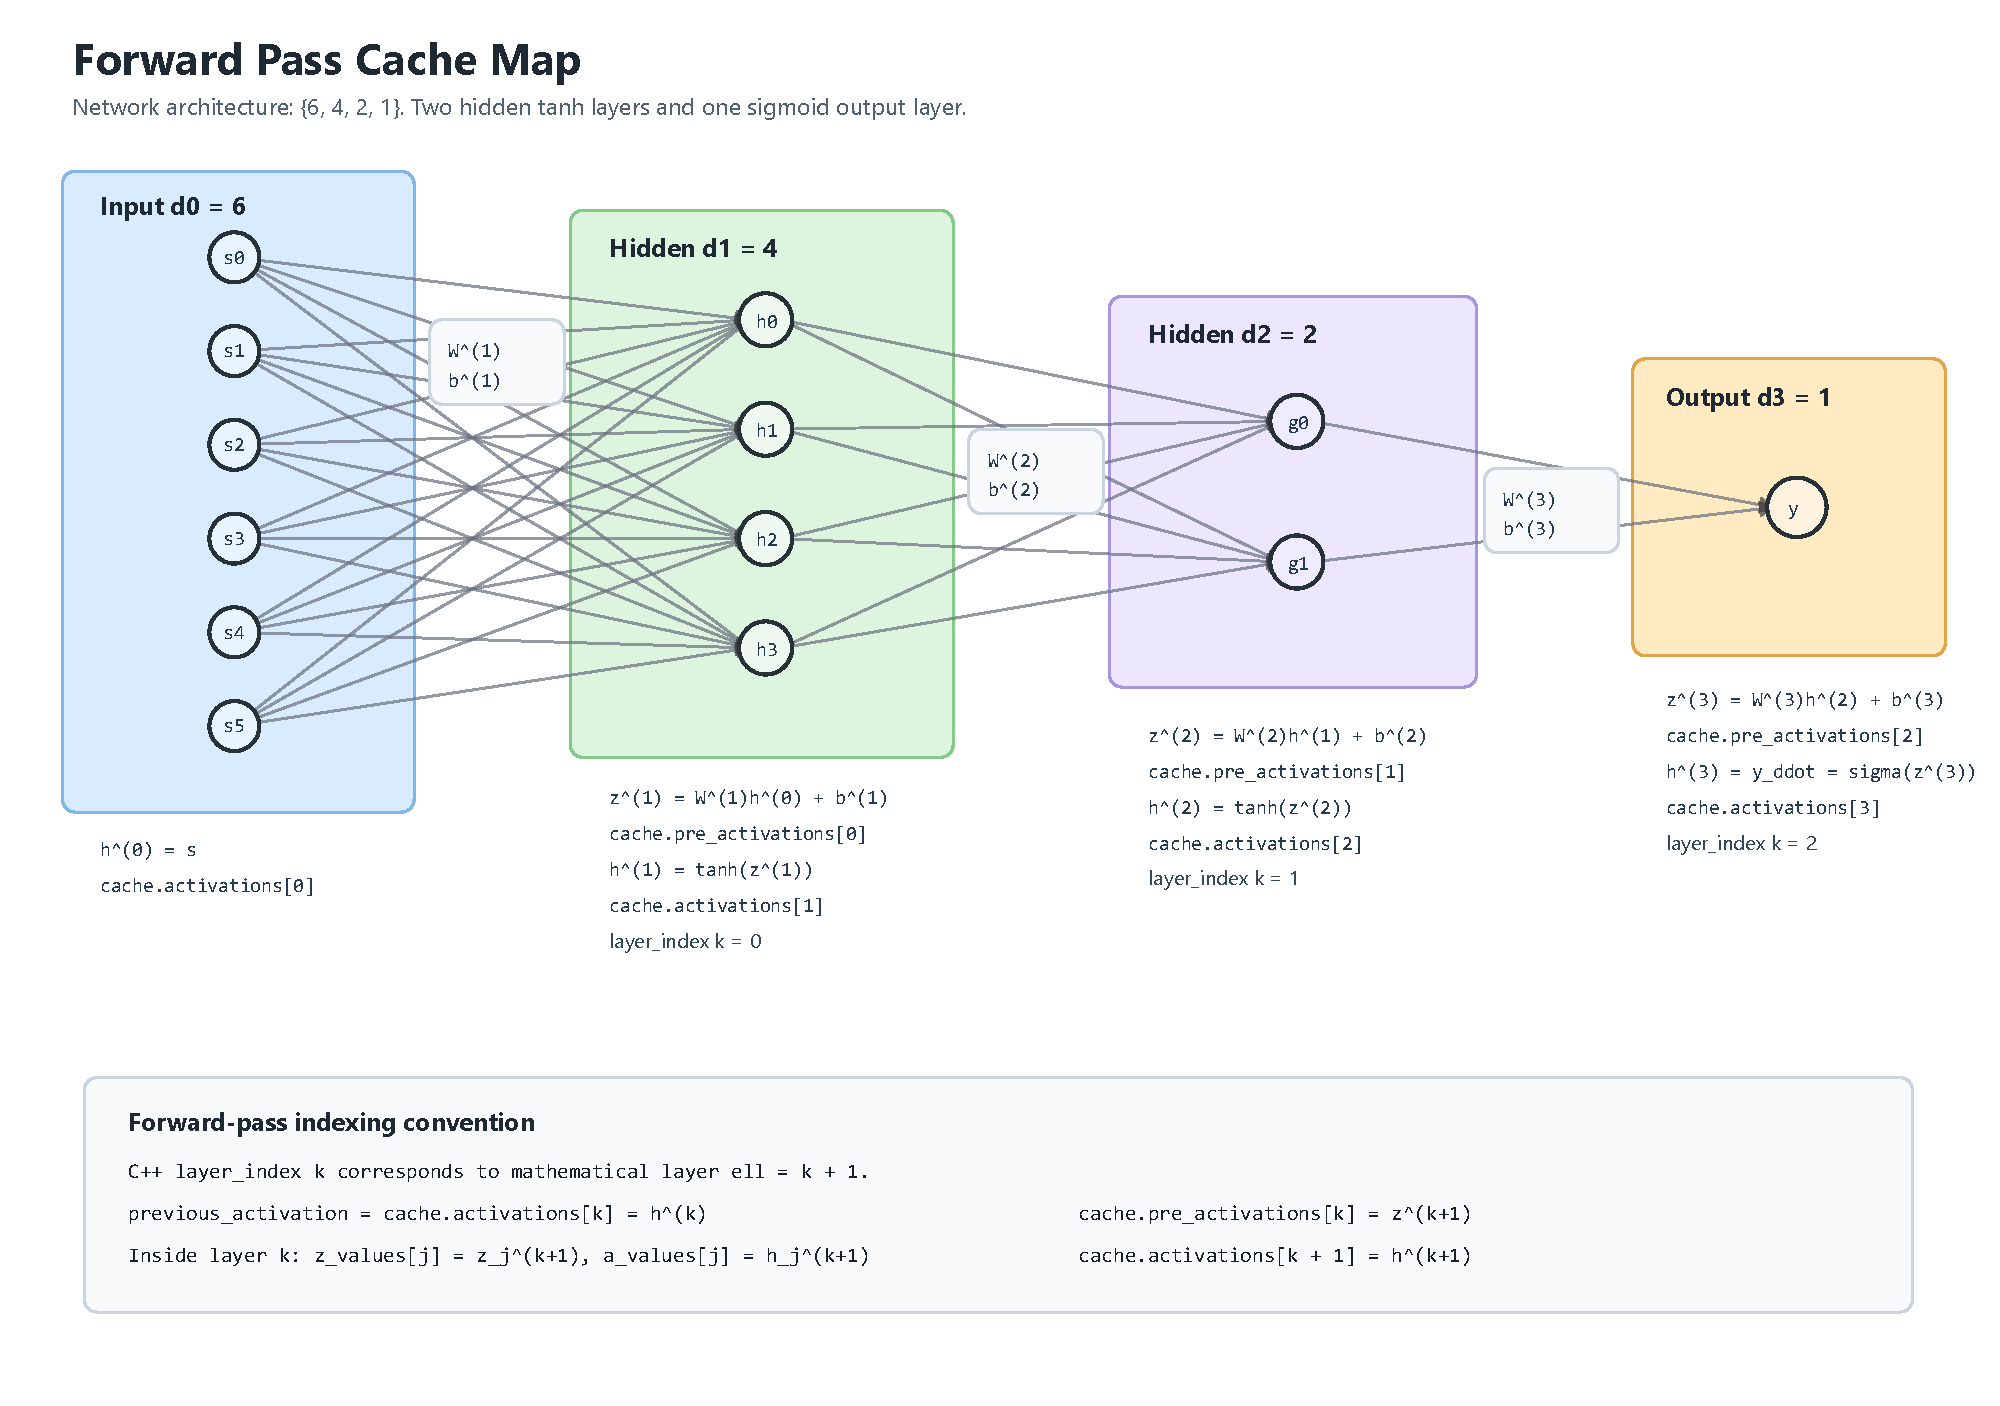
\includegraphics[width=\textwidth]{nn.pdf}
  \caption{Forward-pass cache map for a \(\{6,4,2,1\}\) dense network.
  The diagram shows both mathematical notation, such as
  \(\mathbf{h}^{(k)}\) and \(\mathbf{z}^{(k)}\), and the corresponding C++ cache entries,
  such as \texttt{activations[k]} and \texttt{pre\_activations[k]}.}
  \label{fig:forward-pass-cache-map}
\end{figure}

\section{Stable Binary Cross-Entropy}

\subsection{Bernoulli Maximum-Likelihood Derivation}

For a binary target \(y \in \{0,1\}\), the Bernoulli probability mass
function is
\[
  \Pr(Y=y \mid p) = p^y(1-p)^{1-y},
  \qquad 0 \leq p \leq 1.
\]
The exponents select the appropriate probability: when \(y=1\), this
becomes \(p\); when \(y=0\), it becomes \(1-p\).

For one output unit, the network predicts a probability
\(\hat{y}=\sigma(z)\), where \(z\) is the output logit. Given a dataset
of \(B\) independent training examples, the likelihood of the network
parameters \(\theta\) is
\[
  \mathcal{L}(\theta)
  =
  \prod_{i=1}^{B}
  \left(\hat{y}^{(i)}\right)^{y^{(i)}}
  \left(1-\hat{y}^{(i)}\right)^{1-y^{(i)}},
  \qquad \text{where} \qquad
  \hat{y}^{(i)}=f_\theta\!\left(x^{(i)}\right).
\]
The likelihood above is the maximum-likelihood objective.
\[
  \log \mathcal{L}(\theta)
  =
  \log\!\left[
    \prod_{i=1}^{B}
    \left(\hat{y}^{(i)}\right)^{y^{(i)}}
    \left(1-\hat{y}^{(i)}\right)^{1-y^{(i)}}
  \right].
\]
Because \(\log\) is strictly increasing, this transformation preserves
the maximizing parameters. Next, the rule
\(\log(\prod_i q_i)=\sum_i\log(q_i)\) converts the product into a sum:
\[
  \begin{aligned}
    \log \mathcal{L}(\theta)
    &=
    \sum_{i=1}^{B}
    \left[
      y^{(i)}\log\!\left(\hat{y}^{(i)}\right)
      +
      \left(1-y^{(i)}\right)
      \log\!\left(1-\hat{y}^{(i)}\right)
    \right].
  \end{aligned}
\]
Optimization in this project is written as minimization, so negate the
log-likelihood. The resulting cost for one output unit is the ordinary
binary cross-entropy:
\[
  c_{\mathrm{BCE}}\!\left(\hat{y}, y\right)
  =
  -\left[
    y\log(\hat{y})
    +
    (1-y)\log(1-\hat{y})
  \right].
\]
Thus, maximizing the Bernoulli likelihood and minimizing binary
cross-entropy are the same objective stated in opposite directions. For
the project's terminology, \(c_{\mathrm{BCE}}\) is a per-output-unit cost,
\texttt{sample\_cost} averages those costs across an example's output
units, and \texttt{batch\_loss} averages sample costs across the batch.
The derivation assumes hard Bernoulli observations, \(y \in \{0,1\}\),
although the implementation also accepts targets in \([0,1]\).

\subsection{Logit Substitution for Numerical Stability}

The ordinary expression is mathematically correct, but evaluating it
through \(\hat{y}=\sigma(z)\) can be numerically unsafe when floating
point rounding makes \(\hat{y}\) exactly \(0\) or \(1\). The next part
rewrites the same objective directly in terms of the logit \(z\).

Substitute \(\hat{y}=\sigma(z)\) into ordinary binary cross-entropy.
The sigmoid identities
\[
  \log\!\left(\sigma(z)\right)
  = z-\log\!\left(1+\exp(z)\right)
  \qquad \text{and} \qquad
  \log\!\left(1-\sigma(z)\right)
  =-\log\!\left(1+\exp(z)\right)
\]
give
\[
  \begin{aligned}
    c_{\mathrm{BCE}}(z,y)
    &=
    -y\left[z-\log\!\left(1+\exp(z)\right)\right]
    +(1-y)\log\!\left(1+\exp(z)\right)\\
    &=
    \log\!\left(1+\exp(z)\right)-yz.
  \end{aligned}
\]
This evaluates exactly the same Bernoulli negative log-likelihood as
the probability-space expression; it merely uses the logit directly.
However, the term \(\exp(z)\) can overflow for a large positive logit.
Split the softplus term by the sign of \(z\):
\[
  \log\!\left(1+\exp(z)\right)
  =
  \max(z,0)
  +
  \log\!\left(1+\exp\!\left(-\lvert z\rvert\right)\right).
\]
The stable BCE-from-logit cost is therefore
\[
  c_{\mathrm{BCE}}(z,y)
  =
  \max(z,0)
  -yz
  +
  \log\!\left(1+\exp\!\left(-\lvert z\rvert\right)\right).
\]
The implementation evaluates the final logarithm with
\texttt{std::log1p}, together with \texttt{std::exp} and
\texttt{std::abs}. The numerical reasons for this form and the
corresponding stable sigmoid evaluation are discussed in
Section~\ref{sec:numerical-stability}.

The logit form also gives the useful derivative
\[
  \frac{\partial c_{\mathrm{BCE}}}{\partial z}
  =
  \sigma(z)-y,
\]
which becomes the output-layer error signal in reverse-mode
backpropagation.

\section{Reverse-Mode Backpropagation}

\subsection{Calculus and Linear-Map Foundations}

Reverse-mode backpropagation computes the gradient of a scalar loss with
respect to every trainable parameter by propagating sensitivities with
respect to intermediate variables backward through a composition of
differentiable maps. It is not a new differentiation rule; it is an
efficient organization of the multivariable chain rule.

\paragraph{Scalar Partial Derivatives}
Let \(\mathbf{x}=[x_1,x_2,\ldots,x_n]^\mathsf{T}\in\mathbb{R}^n\). For
a scalar function \(f\), the partial derivative with respect to \(x_j\)
is
\[
  \frac{\partial f}{\partial x_j}(\mathbf{x})
  =
  \lim_{h\to 0}
  \frac{f(\mathbf{x}+h\mathbf{e}_j)-f(\mathbf{x})}{h},
\]
where \(\mathbf{e}_j\) is the coordinate vector with a \(1\) in
position \(j\) and zeros elsewhere. It is the rate of change when only
coordinate \(x_j\) varies.

\paragraph{The Scalar Chain Rule}
Let \(x_0=x\), and suppose a scalar computation forms
\(x_1=f_1(x_0),x_2=f_2(x_1),\ldots,x_R=f_R(x_{R-1})\), with final loss
\(\ell=x_R\). Repeated application of the chain rule gives
\[
  \frac{d\ell}{dx}
  =
  \frac{dx_R}{dx_{R-1}}
  \frac{dx_{R-1}}{dx_{R-2}}
  \cdots
  \frac{dx_1}{dx_0}.
\]
The two-function form \(\ell=f(u)\), \(u=g(x)\) is the special case
\(R=2\). This product structure is the scalar prototype for reverse
mode: begin with the derivative of the loss at the output, then
multiply by local derivatives while moving backward through the
computation.

More generally, let the scalar output be \(z=f(u_1,\ldots,u_m)\), where
each intermediate variable \(u_j\) depends on
\(\mathbf{x}=[x_1,\ldots,x_n]^\mathsf{T}\). The partial derivative with
respect to input component \(x_k\) sums every intermediate contribution:
\[
  \frac{\partial z}{\partial x_k}
  =
  \sum_{j=1}^{m}
  \frac{\partial z}{\partial u_j}
  \frac{\partial u_j}{\partial x_k}.
\]

\paragraph{Gradients of Scalar-Valued Functions}
For a differentiable scalar function \(f:\mathbb{R}^n\to\mathbb{R}\),
the gradient collects all first partial derivatives into a column vector:
\[
  \nabla f(\mathbf{x})
  =
  \begin{bmatrix}
    \dfrac{\partial f}{\partial x_1} &
    \dfrac{\partial f}{\partial x_2} &
    \cdots &
    \dfrac{\partial f}{\partial x_n}
  \end{bmatrix}^{\mathsf{T}}
  \in\mathbb{R}^n.
\]
For a small perturbation \(\Delta\mathbf{x}\), the gradient gives the
first-order change
\[
  f(\mathbf{x}+\Delta\mathbf{x})
  =
  f(\mathbf{x})
  +
  \nabla f(\mathbf{x})^\mathsf{T}\Delta\mathbf{x}
  +
  o\bigl(\lVert\Delta\mathbf{x}\rVert\bigr).
\]

\paragraph{Total Derivatives, Differentials, and Gradients}
For a differentiable map
\(\mathbf{F}:\mathbb{R}^n\to\mathbb{R}^m\), the total derivative at
\(\mathbf{x}\) is the linear map
\[
  D\mathbf{F}(\mathbf{x}):\mathbb{R}^n\to\mathbb{R}^m
\]
satisfying
\[
  \mathbf{F}(\mathbf{x}+\Delta\mathbf{x})
  =
  \mathbf{F}(\mathbf{x})
  +
  D\mathbf{F}(\mathbf{x})[\Delta\mathbf{x}]
  +
  o\bigl(\lVert\Delta\mathbf{x}\rVert\bigr).
\]
In standard coordinates, this derivative is represented by the
Jacobian
\[
  \mathbf{J}_{\mathbf{F}}(\mathbf{x})
  =
  \left[
    \frac{\partial F_i}{\partial x_j}(\mathbf{x})
  \right]_{i=1,\ldots,m;\,j=1,\ldots,n}
  \in\mathbb{R}^{m\times n},
\]
whose action is
\[
  D\mathbf{F}(\mathbf{x})[\Delta\mathbf{x}]
  =
  \mathbf{J}_{\mathbf{F}}(\mathbf{x})\Delta\mathbf{x}.
\]

For a scalar loss \(L:\mathbb{R}^m\to\mathbb{R}\), its differential at
\(\mathbf{y}\) is the linear functional
\(dL_{\mathbf{y}}[\Delta\mathbf{y}]\). Under the Euclidean inner
product, the gradient is the unique column vector satisfying
\[
  dL_{\mathbf{y}}[\Delta\mathbf{y}]
  =
  \left\langle\nabla_{\mathbf{y}}L,\Delta\mathbf{y}\right\rangle
  =
  (\nabla_{\mathbf{y}}L)^\mathsf{T}\Delta\mathbf{y}.
\]
Thus, the derivative or differential is intrinsically a linear map or
linear functional, while the gradient is its vector representation
under the chosen Euclidean inner product.

\paragraph{Componentwise and Vector Chain Rules}
For the vector-valued composition
\(\mathbf{h}(\mathbf{x})=\mathbf{f}(\mathbf{g}(\mathbf{x}))\), let
\(\mathbf{x}\in\mathbb{R}^n\), \(\mathbf{g}(\mathbf{x})\in\mathbb{R}^m\),
and \(\mathbf{h}(\mathbf{x})\in\mathbb{R}^p\). The derivative of output
component \(h_i\) with respect to input component \(x_k\) is
\[
  \frac{\partial h_i}{\partial x_k}
  =
  \sum_{j=1}^{m}
  \frac{\partial f_i}{\partial g_j}
  \frac{\partial g_j}{\partial x_k}.
\]
In matrix form, the same rule is
\[
  \mathbf{J}_{\mathbf{h}}(\mathbf{x})
  =
  \mathbf{J}_{\mathbf{f}}\bigl(\mathbf{g}(\mathbf{x})\bigr)
  \mathbf{J}_{\mathbf{g}}(\mathbf{x}).
\]
The indexed expression exposes the sum over intermediate components;
the Jacobian expression collects all of those componentwise
derivatives into one matrix equation.

\paragraph{Adjoints and Reverse Mode}
Let \(\mathbf{y}=\mathbf{F}(\mathbf{x})\). Applying the preceding
definitions to a scalar loss gives
\[
  \begin{aligned}
    d(L\circ\mathbf{F})_{\mathbf{x}}[\Delta\mathbf{x}]
    &=
    dL_{\mathbf{y}}
    \left[
      D\mathbf{F}(\mathbf{x})[\Delta\mathbf{x}]
    \right]\\
    &=
    \left\langle
      \nabla_{\mathbf{y}}L,
      D\mathbf{F}(\mathbf{x})[\Delta\mathbf{x}]
    \right\rangle\\
    &=
    \left\langle
      D\mathbf{F}(\mathbf{x})^*\nabla_{\mathbf{y}}L,
      \Delta\mathbf{x}
    \right\rangle.
  \end{aligned}
\]
Therefore,
\[
  \boxed{
    \nabla_{\mathbf{x}}(L\circ\mathbf{F})
    =
    D\mathbf{F}(\mathbf{x})^*
    \nabla_{\mathbf{y}}L
  }
\]
and, in standard Euclidean coordinates,
\[
  \boxed{
    \nabla_{\mathbf{x}}(L\circ\mathbf{F})
    =
    \mathbf{J}_{\mathbf{F}}(\mathbf{x})^\mathsf{T}
    \nabla_{\mathbf{y}}L.
  }
\]
Forward differentiation pushes perturbations forward through derivative
maps. Reverse-mode differentiation pulls loss sensitivities backward
through the adjoints of those maps. This backward action is the
\emph{pullback} in the concrete finite-dimensional sense used here; in
Euclidean coordinates, the adjoints are represented by transpose
Jacobians.

\paragraph{Matrix Gradients for Scalar Losses}
For a scalar loss \(L\) and matrix parameter
\(\mathbf{X}\in\mathbb{R}^{r\times s}\), define
\[
  \left[\nabla_{\mathbf{X}}L\right]_{ij}
  \equiv
  \frac{\partial L}{\partial X_{ij}}.
\]
The associated differential is characterized by the Frobenius inner
product:
\[
  \boxed{
    dL
    =
    \left\langle\nabla_{\mathbf{X}}L,d\mathbf{X}\right\rangle_F
    =
    \operatorname{tr}
    \left(
      (\nabla_{\mathbf{X}}L)^\mathsf{T}d\mathbf{X}
    \right).
  }
\]
Matrix-derivative arrangements differ across sources, so formulas
derived under incompatible conventions should not be mixed. The
scalar-loss convention above is the one used throughout the
backpropagation derivation; see \cite{golden2020} for a fuller discussion of related
matrix-calculus conventions.

\subsection{Reverse-Mode Backpropagation for the MLP}

For one input-target pair, the backward pass computes its parameter
gradient in three stages:
\begin{enumerate}
  \item Compute the output-layer sensitivity from the cached sigmoid
  output and its target.
  \item Transport that sensitivity backward through every hidden layer,
  multiplying by the relevant weights and local activation derivatives.
  \item Turn each layer's sensitivity into its bias gradient and
  weight-gradient matrix.
\end{enumerate}

\paragraph{Reverse Accumulation on a Computational Graph}
The neural network is a directed acyclic computational graph. For each
intermediate vector node \(\mathbf{u}\), define its reverse sensitivity,
or adjoint, by
\[
  \overline{\mathbf{u}}
  \equiv
  \nabla_{\mathbf{u}}L.
\]
The reverse pass begins at the scalar loss with
\[
  \overline{L}=1.
\]
If \(\mathbf{u}\) influences multiple child nodes \(\mathbf{v}\), its
total reverse sensitivity is
\[
  \boxed{
    \overline{\mathbf{u}}
    =
    \sum_{\mathbf{v}\in\operatorname{children}(\mathbf{u})}
    \mathbf{J}_{\mathbf{v},\mathbf{u}}^\mathsf{T}
    \overline{\mathbf{v}}.
  }
\]
Backpropagation evaluates this recursion in reverse topological order.
It applies Jacobian transposes to sensitivities without materializing
full Jacobians. This reuse of already-computed sensitivities is the
dynamic-programming aspect that makes reverse-mode differentiation
practical for this MLP.

\paragraph{Network and Parameter Notation}
Let the architecture have widths \(d_0,d_1,\ldots,d_M\), where \(d_0\)
is the number of input units, \(d_M\) is the number of output units, and
\(M-1\) is an arbitrary number of hidden layers. Let
\[
  \boldsymbol\theta
  =
  \left\{
    \bigl(\mathbf{W}^{(k)},\mathbf{b}^{(k)}\bigr)
  \right\}_{k=1}^{M},
  \qquad
  \mathbf{W}^{(k)}\in\mathbb{R}^{d_k\times d_{k-1}},
  \qquad
  \mathbf{b}^{(k)}\in\mathbb{R}^{d_k}.
\]
For an input pattern \(\mathbf{s}\in\mathbb{R}^{d_0}\), the network
begins with
\[
  \mathbf{h}^{(0)}=\mathbf{s}.
\]
For every hidden layer \(k=1,\ldots,M-1\), this project uses a dense
affine transformation followed by componentwise \(\tanh\):
\[
  \mathbf{z}^{(k)}
  =
  \mathbf{W}^{(k)}\mathbf{h}^{(k-1)}
  +
  \mathbf{b}^{(k)},
  \qquad
  \mathbf{h}^{(k)}
  =
  \tanh\bigl(\mathbf{z}^{(k)}\bigr).
\]
The final dense layer uses the same affine transformation but applies
the sigmoid componentwise:
\[
  \mathbf{z}^{(M)}
  =
  \mathbf{W}^{(M)}\mathbf{h}^{(M-1)}
  +
  \mathbf{b}^{(M)},
  \qquad
  \mathbf{h}^{(M)}
  =
  \sigma\bigl(\mathbf{z}^{(M)}\bigr),
\]
\[
  \ddot{\mathbf{y}}(\mathbf{s},\boldsymbol\theta)
  =
  \mathbf{h}^{(M)}.
\]
This notation also covers a network with no hidden layers: when
\(M=1\), the hidden-layer equations are absent and the input feeds
directly into the sigmoid output layer. Although
\(\boldsymbol\theta\) is displayed as a collection of layer parameters,
\(\nabla_{\boldsymbol\theta}L\) denotes the column vector obtained by
concatenating all scalar parameter derivatives in one fixed order
consistent with the implementation's storage convention.

\paragraph{Sample Loss and Output Sensitivity}
For one input-target pair with
\(\mathbf{y}\in[0,1]^{d_M}\), let \(L\) be the mean binary
cross-entropy from logits across independent output units:
\[
  L
  =
  \frac{1}{d_M}
  \sum_{j=1}^{d_M}
  c_{\mathrm{BCE}}\left(z_j^{(M)},y_j\right).
\]
Here \(c_{\mathrm{BCE}}\) is the scalar binary cross-entropy cost
defined in the preceding section and evaluated from a logit using its
numerically stable form. Define the layer sensitivity by
\[
  \boldsymbol{\delta}^{(k)}
  \equiv
  \nabla_{\mathbf{z}^{(k)}}L,
  \qquad
  k=1,\ldots,M.
\]

\paragraph{Interpreting a Layer Sensitivity}
Componentwise, the \(j\)-th sensitivity is
\[
  \delta_j^{(k)}
  =
  \frac{\partial L}{\partial z_j^{(k)}}.
\]
It is called a sensitivity because it measures how responsive the final
loss is to a small change in the preactivation of neuron \(j\). More
precisely, if only \(z_j^{(k)}\) is perturbed by a small amount
\(\epsilon\), then
\[
  L\!\left(
    \mathbf{z}^{(k)}+\epsilon\mathbf{e}_j
  \right)
  =
  L\!\left(\mathbf{z}^{(k)}\right)
  +
  \delta_j^{(k)}\epsilon
  +
  o\!\left(\lvert\epsilon\rvert\right).
\]
Consequently, for a small positive perturbation:
\begin{itemize}
  \item if \(\delta_j^{(k)}>0\), increasing \(z_j^{(k)}\) increases the
  loss locally;
  \item if \(\delta_j^{(k)}<0\), increasing \(z_j^{(k)}\) decreases the
  loss locally;
  \item if \(\lvert\delta_j^{(k)}\rvert\) is large, the loss is highly
  responsive to that preactivation; and
  \item if \(\delta_j^{(k)}\approx0\), the loss is locally insensitive
  to it.
\end{itemize}
Thus, a sensitivity is not a quantity separate from calculus: it is a
partial derivative. It receives its own symbol because the same
downstream derivative is reused repeatedly when backpropagation
transports information through a layer and forms the gradients of all
of that layer's weights and biases.

Because a sigmoid output paired with binary cross-entropy has derivative
\(\sigma(z)-y\), the output sensitivity is
\[
  \boxed{
    \boldsymbol{\delta}^{(M)}
    =
    \frac{\mathbf{h}^{(M)}-\mathbf{y}}{d_M}.
  }
\]
The factor \(1/d_M\) appears because this implementation averages the
binary cross-entropy across output units.

\paragraph{Differential Derivation for One Affine Layer}
Consider one generic affine layer,
\[
  \mathbf{z}
  =
  \mathbf{W}\mathbf{h}+\mathbf{b},
  \qquad
  \boldsymbol{\delta}
  =
  \nabla_{\mathbf{z}}L.
\]
Its perturbation is
\[
  d\mathbf{z}
  =
  (d\mathbf{W})\mathbf{h}
  +
  \mathbf{W}\,d\mathbf{h}
  +
  d\mathbf{b}.
\]
Consequently,
\[
  \begin{aligned}
    dL
    &=
    \boldsymbol{\delta}^\mathsf{T}d\mathbf{z}\\
    &=
    \boldsymbol{\delta}^\mathsf{T}(d\mathbf{W})\mathbf{h}
    +
    \boldsymbol{\delta}^\mathsf{T}\mathbf{W}\,d\mathbf{h}
    +
    \boldsymbol{\delta}^\mathsf{T}d\mathbf{b}.
  \end{aligned}
\]
The term involving the previous activation is
\[
  \boldsymbol{\delta}^\mathsf{T}\mathbf{W}\,d\mathbf{h}
  =
  (\mathbf{W}^\mathsf{T}\boldsymbol{\delta})^\mathsf{T}d\mathbf{h},
\]
so
\[
  \boxed{
    \nabla_{\mathbf{h}}L
    =
    \mathbf{W}^\mathsf{T}\boldsymbol{\delta}.
  }
  \qquad
  \boxed{
    \nabla_{\mathbf{b}}L
    =
    \boldsymbol{\delta}.
  }
\]
For the weight term, the trace/Frobenius identity gives
\[
  \begin{aligned}
    \boldsymbol{\delta}^\mathsf{T}(d\mathbf{W})\mathbf{h}
    &=
    \operatorname{tr}
    \left(
      \boldsymbol{\delta}^\mathsf{T}(d\mathbf{W})\mathbf{h}
    \right)\\
    &=
    \operatorname{tr}
    \left(
      \mathbf{h}\boldsymbol{\delta}^\mathsf{T}d\mathbf{W}
    \right)\\
    &=
    \operatorname{tr}
    \left(
      (\boldsymbol{\delta}\mathbf{h}^\mathsf{T})^\mathsf{T}
      d\mathbf{W}
    \right).
  \end{aligned}
\]
Therefore,
\[
  \boxed{
    \nabla_{\mathbf{W}}L
    =
    \boldsymbol{\delta}\mathbf{h}^\mathsf{T}.
  }
\]
The outer product appears because each weight \(W_{ji}\) multiplies the
input activation \(h_i\) and contributes to output preactivation
\(z_j\).

\paragraph{Activation Pullback and Hidden-Layer Recursion}
For a general elementwise hidden activation
\(\boldsymbol{\phi}_k\), its Jacobian is
\[
  \mathbf{J}_{\boldsymbol{\phi}_k}(\mathbf{z}^{(k)})
  =
  \operatorname{DIAG}
  \left(
    \boldsymbol{\phi}_k'(\mathbf{z}^{(k)})
  \right).
\]
The hidden sensitivity is
\[
  \boxed{
    \boldsymbol{\delta}^{(k)}
    =
    \mathbf{J}_{\boldsymbol{\phi}_k}(\mathbf{z}^{(k)})^\mathsf{T}
    (\mathbf{W}^{(k+1)})^\mathsf{T}
    \boldsymbol{\delta}^{(k+1)},
    \qquad
    k=M-1,\ldots,1.
  }
\]
For an elementwise activation, this is
\[
  \boldsymbol{\delta}^{(k)}
  =
  \left(
    (\mathbf{W}^{(k+1)})^\mathsf{T}
    \boldsymbol{\delta}^{(k+1)}
  \right)
  \odot
  \boldsymbol{\phi}_k'(\mathbf{z}^{(k)}).
\]
Here \(\boldsymbol{\phi}_k=\tanh\), so
\[
  \boldsymbol{\phi}_k'(\mathbf{z}^{(k)})
  =
  \mathbf{1}-(\mathbf{h}^{(k)})^2
\]
componentwise. The recursion used by this network is therefore
\[
  \boxed{
    \boldsymbol{\delta}^{(k)}
    =
    \left(
      (\mathbf{W}^{(k+1)})^\mathsf{T}
      \boldsymbol{\delta}^{(k+1)}
    \right)
    \odot
    \left(
      \mathbf{1}-(\mathbf{h}^{(k)})^2
    \right).
  }
\]
Once the sensitivity is known, the gradients of layer \(k\)'s affine
parameters are
\[
  \boxed{
    \nabla_{\mathbf{W}^{(k)}}L
    =
    \boldsymbol{\delta}^{(k)}
    (\mathbf{h}^{(k-1)})^\mathsf{T},
    \qquad
    \nabla_{\mathbf{b}^{(k)}}L
    =
    \boldsymbol{\delta}^{(k)}.
  }
\]
The componentwise matrix-gradient arrangement is
\[
  \left[
    \nabla_{\mathbf{W}^{(k)}}L
  \right]_{ji}
  \equiv
  \frac{\partial L}{\partial W_{ji}^{(k)}}
  =
  \delta_j^{(k)}h_i^{(k-1)}.
\]

\paragraph{Corresponding C++ backward pass}
The following is the computational core of \texttt{backward} from this project. The input-validation call is omitted here so that the relationship between the code and the preceding equations is easier to see.

\begin{lstlisting}[language=C++]
NetworkGradients backward(
    const MLP& network,
    const ForwardCache& cache,
    const Values& target
)
{
    NetworkGradients gradients = make_zero_gradients_like(network);

    std::vector<Values> deltas;
    deltas.reserve(network.layers.size());
    for (const DenseLayer& layer : network.layers) {
        deltas.emplace_back(layer.output_size, 0.0);
    }

    const std::size_t output_layer_index = network.layers.size() - 1;
    const std::size_t output_width =
        network.layers[output_layer_index].output_size;
    const Values& output_activation =
        cache.activations[output_layer_index + 1];

    // [1] Output sensitivity: delta^M = (h^M - y) / d_M.
    for (std::size_t j = 0; j < output_width; ++j) {
        deltas[output_layer_index][j] =
            (output_activation[j] - target[j]) /
            static_cast<double>(output_width);
    }

    // [2] Transport delta backward and apply the tanh derivative.
    for (std::size_t next_layer_index = output_layer_index;
         next_layer_index > 0;
         --next_layer_index) {
        const std::size_t layer_index = next_layer_index - 1;
        const DenseLayer& layer = network.layers[layer_index];
        const DenseLayer& next_layer = network.layers[next_layer_index];
        const Values& activation = cache.activations[layer_index + 1];

        for (std::size_t j = 0; j < layer.output_size; ++j) {
            double transported_delta = 0.0;

            for (std::size_t r = 0; r < next_layer.output_size; ++r) {
                transported_delta +=
                    next_layer.weight(r, j) *
                    deltas[next_layer_index][r];
            }

            const double tanh_derivative =
                1.0 - activation[j] * activation[j];
            deltas[layer_index][j] =
                transported_delta * tanh_derivative;
        }
    }

    // [3] Turn every delta into bias and weight gradients.
    for (std::size_t layer_index = 0;
         layer_index < network.layers.size();
         ++layer_index) {
        const DenseLayer& layer = network.layers[layer_index];
        const Values& previous_activation =
            cache.activations[layer_index];
        LayerGradients& layer_gradients = gradients.layers[layer_index];

        for (std::size_t j = 0; j < layer.output_size; ++j) {
            layer_gradients.biases[j] = deltas[layer_index][j];

            for (std::size_t i = 0; i < layer.input_size; ++i) {
                layer_gradients.weights[j * layer.input_size + i] =
                    deltas[layer_index][j] * previous_activation[i];
            }
        }
    }

    return gradients;
}
\end{lstlisting}

\paragraph{Code-to-equation map}
The C++ layer index \texttt{layer\_index} is zero-based, so it
represents mathematical layer \(k=\texttt{layer\_index}+1\).
Accordingly, \texttt{cache.activations[layer\_index]} is
\(\mathbf{h}^{(k-1)}\), while
\texttt{cache.activations[layer\_index + 1]} is \(\mathbf{h}^{(k)}\).
\begin{enumerate}
  \item Region \texttt{[1]} reads the final cached activation
  \(\mathbf{h}^{(M)}\) and implements
  \(\boldsymbol{\delta}^{(M)}
  =(\mathbf{h}^{(M)}-\mathbf{y})/d_M\). The division by
  \texttt{output\_width} is the mean over output units in the
  per-pattern loss.
  \item Region \texttt{[2]} accumulates one coordinate of
  \((\mathbf{W}^{(k+1)})^\mathsf{T}
  \boldsymbol{\delta}^{(k+1)}\) in \texttt{transported\_delta}. The
  next two lines multiply it by
  \(1-h_j^{(k)}h_j^{(k)}\), applying the local \(\tanh\) derivative to
  produce the \(j\)-th component of
  \(\boldsymbol{\delta}^{(k)}\).
  \item Region \texttt{[3]} implements
  \(\nabla_{\mathbf{b}^{(k)}}L=\boldsymbol{\delta}^{(k)}\) by assigning
  each bias gradient directly. Its innermost assignment implements
  \([\nabla_{\mathbf{W}^{(k)}}L]_{ji}
  =\delta_j^{(k)}h_i^{(k-1)}\);
  \texttt{j * layer.input\_size + i} is the row-major storage offset for
  matrix entry \((j,i)\).
\end{enumerate}
The code does not create the diagonal activation Jacobian. It applies
that Jacobian's action efficiently through componentwise multiplication.

\paragraph{Backpropagation and Gradient Descent}
For one training pattern, backpropagation computes
\[
  \nabla_{\boldsymbol\theta}L_n(\boldsymbol\theta).
\]
It does not update the parameters. A separate optimization algorithm
combines one or more such gradients and chooses a parameter update.
Conceptually, backpropagation is an efficient reverse-order organization
of the chain rule that reuses downstream derivatives rather than
recomputing them separately for every parameter.

\section{Full-Batch Empirical Risk Gradient}

For \(N\) training patterns, the full-batch empirical-risk objective is
\[
  \widehat{\ell}_N(\boldsymbol\theta)
  =
  \frac{1}{N}
  \sum_{n=1}^{N}
  L_n(\boldsymbol\theta).
\]
Linearity of differentiation gives the matching full-batch gradient:
\[
  \nabla_{\boldsymbol\theta}
  \widehat{\ell}_N(\boldsymbol\theta)
  =
  \frac{1}{N}
  \sum_{n=1}^{N}
  \nabla_{\boldsymbol\theta}L_n(\boldsymbol\theta).
\]
Full-batch gradient descent first computes this average and then applies
the update
\[
  \boxed{
    \boldsymbol\theta^{(t+1)}
    =
    \boldsymbol\theta^{(t)}
    -
    \gamma_t
    \nabla_{\boldsymbol\theta}
    \widehat{\ell}_N\left(\boldsymbol\theta^{(t)}\right).
  }
\]
Thus, backpropagation produces a per-pattern gradient, while the
full-batch optimizer averages those gradients before changing the
parameters.

\subsection{Example: Full-Batch XOR Objective for a 2-4-1 Network}

Consider the XOR dataset, written as four input-target pairs:
\[
  \begin{aligned}
    (\mathbf{s}_1,y_1)&=((0,0)^\mathsf{T},0),&
    (\mathbf{s}_2,y_2)&=((0,1)^\mathsf{T},1),\\
    (\mathbf{s}_3,y_3)&=((1,0)^\mathsf{T},1),&
    (\mathbf{s}_4,y_4)&=((1,1)^\mathsf{T},0).
  \end{aligned}
\]
For the \(\{2,4,1\}\) architecture, \(d_0=2\), \(d_1=4\), and
\(d_2=1\). Its parameter collection is
\[
  \boldsymbol\theta
  =
  \left\{
    \mathbf{W}^{(1)},\mathbf{b}^{(1)},
    \mathbf{W}^{(2)},\mathbf{b}^{(2)}
  \right\},
\]
with
\[
  \mathbf{W}^{(1)}\in\mathbb{R}^{4\times 2},
  \quad
  \mathbf{b}^{(1)}\in\mathbb{R}^{4},
  \quad
  \mathbf{W}^{(2)}\in\mathbb{R}^{1\times 4},
  \quad
  \mathbf{b}^{(2)}\in\mathbb{R}^{1}.
\]
There are \(4\cdot2+4+1\cdot4+1=17\) scalar parameters. For pattern
\(n\), the forward computation is
\[
  \begin{aligned}
    \mathbf{h}_n^{(0)}&=\mathbf{s}_n,\\
    \mathbf{z}_n^{(1)}
    &=
    \mathbf{W}^{(1)}\mathbf{s}_n+\mathbf{b}^{(1)},&
    \mathbf{h}_n^{(1)}
    &=
    \tanh\bigl(\mathbf{z}_n^{(1)}\bigr),\\
    \mathbf{z}_n^{(2)}
    &=
    \mathbf{W}^{(2)}\mathbf{h}_n^{(1)}+\mathbf{b}^{(2)},&
    \ddot{y}_n
    &=
    \sigma\bigl(z_n^{(2)}\bigr).
  \end{aligned}
\]
The output is one-dimensional, so averaging across output units changes
nothing. The sample loss is simply
\[
  L_n
  =
  c_{\mathrm{BCE}}\bigl(z_n^{(2)},y_n\bigr),
\]
and the full-batch XOR objective is
\[
  \widehat{\ell}_4(\boldsymbol\theta)
  =
  \frac{1}{4}
  \sum_{n=1}^{4}
  c_{\mathrm{BCE}}\bigl(z_n^{(2)},y_n\bigr).
\]

The per-pattern output and hidden sensitivities are
\[
  \boldsymbol{\delta}_n^{(2)}
  =
  \ddot{y}_n-y_n,
  \qquad
  \boldsymbol{\delta}_n^{(1)}
  =
  \left(
    (\mathbf{W}^{(2)})^\mathsf{T}
    \boldsymbol{\delta}_n^{(2)}
  \right)
  \odot
  \left(
    \mathbf{1}-(\mathbf{h}_n^{(1)})^2
  \right).
\]
Applying the affine-layer gradient rule to all four patterns and then
averaging gives
\[
  \begin{aligned}
    \nabla_{\mathbf{W}^{(1)}}\widehat{\ell}_4
    &=
    \frac{1}{4}
    \sum_{n=1}^{4}
    \boldsymbol{\delta}_n^{(1)}\mathbf{s}_n^\mathsf{T},&
    \nabla_{\mathbf{b}^{(1)}}\widehat{\ell}_4
    &=
    \frac{1}{4}
    \sum_{n=1}^{4}
    \boldsymbol{\delta}_n^{(1)},\\
    \nabla_{\mathbf{W}^{(2)}}\widehat{\ell}_4
    &=
    \frac{1}{4}
    \sum_{n=1}^{4}
    \boldsymbol{\delta}_n^{(2)}
    (\mathbf{h}_n^{(1)})^\mathsf{T},&
    \nabla_{\mathbf{b}^{(2)}}\widehat{\ell}_4
    &=
    \frac{1}{4}
    \sum_{n=1}^{4}
    \boldsymbol{\delta}_n^{(2)}.
  \end{aligned}
\]
The implementation can therefore run a forward pass and
\texttt{backward} once for each XOR pair, add the four gradient
structures componentwise, divide every accumulated entry by \(4\), and
only then apply one parameter update.

\section{Numerical Stability and Computational Complexity}
\label{sec:numerical-stability}

% Discuss stable sigmoid evaluation for large positive or negative logits.
% Discuss stable BCE-with-logits evaluation and avoidance of log(0).
% Check parameters, activations, losses, and gradients for NaN or infinity.
%
% Explain finite-precision concerns such as cancellation and overflow. Analyze using Taylor series error
%
% Talk about sigmoid and tanh rewrites
% Talk about using log1p as opposed to regular log, talk about stable logit formula
%
% Parameter count:
% P = \sum_{\ell=1}^{L}
%     (n_\ell n_{\ell-1} + n_\ell).
%
% Single-example forward-pass cost:
% O(\sum_{\ell=1}^{L} n_\ell n_{\ell-1}).
%
% Backpropagation has the same asymptotic order.
% A full-batch iteration multiplies this cost by m.
%
% Central finite differences require approximately 2P full objective
% evaluations, making them much more expensive than backpropagation.
%
% Mention memory required to store parameters, gradients,
% activations, and preactivations.

\section{Iterative Descent Optimization and Step Size Selection}

% Define the update:
% \theta_{t+1}
% = \theta_t - \eta\nabla J(\theta_t).
%
% Explain why -\nabla J is the direction of steepest local decrease
% under the Euclidean norm.
%
% Define \eta as the learning rate.
% Clearly distinguish \eta from the finite-difference perturbation h.
%
% Explain:
% small \eta -> stable but slow progress,
% large \eta -> overshooting, oscillation, or divergence.
%
% State whether a fixed learning rate is used.
% Record stopping criteria and maximum iteration count.
%
% Optionally include the descent-lemma result:
% if the gradient is L-Lipschitz, then a step with
% 0 < \eta < 2/L produces local descent when the gradient is nonzero.
%
% Clarify that the neural-network loss is nonconvex, so this does not
% guarantee convergence to a global minimum.
% Talk about Wolfe Step Size Conditions & Downhill condition in deterministic nonlinear optimization theory & Zoutendijk-Wolfe Convergence Theorem
%

\section{Experimental Results}

% State the exact XOR architecture, for example 2 -> 2 -> 1.
% Record activation functions, seed, learning rate,
% finite-difference step, tolerance, and iteration count.
%
% Report:
% initial loss,
% final loss,
% final gradient norm,
% maximum gradient-check error,
% and whether training was deterministic.
%
% Give predicted probabilities for all four XOR inputs.
% Convert probabilities to classes using threshold 0.5.
%
% Include a loss-versus-iteration graph if useful.
% Discuss successful learning and any failed learning-rate
% or architecture configurations.

\section{Limitations and Possible Extensions}

% Limitations:
% tiny XOR dataset,
% only fully connected layers,
% full-batch training,
% binary classification,
% basic gradient descent,
% CPU-only scalar implementation,
% and no production-focused tensor library.
%
% Possible extensions:
% mini-batch or stochastic gradient descent,
% momentum or Adam,
% multiclass softmax and cross-entropy,
% additional activation functions,
% regularization,
% train-validation splits,
% serialization,
% vectorization or multithreading,
% and GPU/CUDA support.
%
% Mention that finite-difference checking is suitable for testing
% small networks but is too expensive for normal training.

\begin{thebibliography}{9}
\bibitem{golden2020}
Richard M. Golden.
\textit{Statistical Machine Learning: A Unified Framework}.
CRC Press, 2020.
\end{thebibliography}

\end{document}
